% Optional: compiles a single PDF of layout reference scans (third-party sample resumes).
% Rename the image files on disk to match \includegraphics paths below after mv.

\documentclass[11pt]{article}

\usepackage[margin=0.75in]{geometry}
\usepackage{graphicx}
\usepackage{caption}

\pagestyle{empty}
\captionsetup{font=small,labelfont=bf}

\begin{document}

\begin{center}
    {\Large \textbf{Layout reference scans}}\\
    \vspace{0.25em}
    {\small Personal LaTeX sources for Jade Zhao are \texttt{jade-zhao-*.tex}; these images are external samples kept for formatting ideas only.}
\end{center}

\vspace{1em}

\begin{figure}[p]
    \centering
    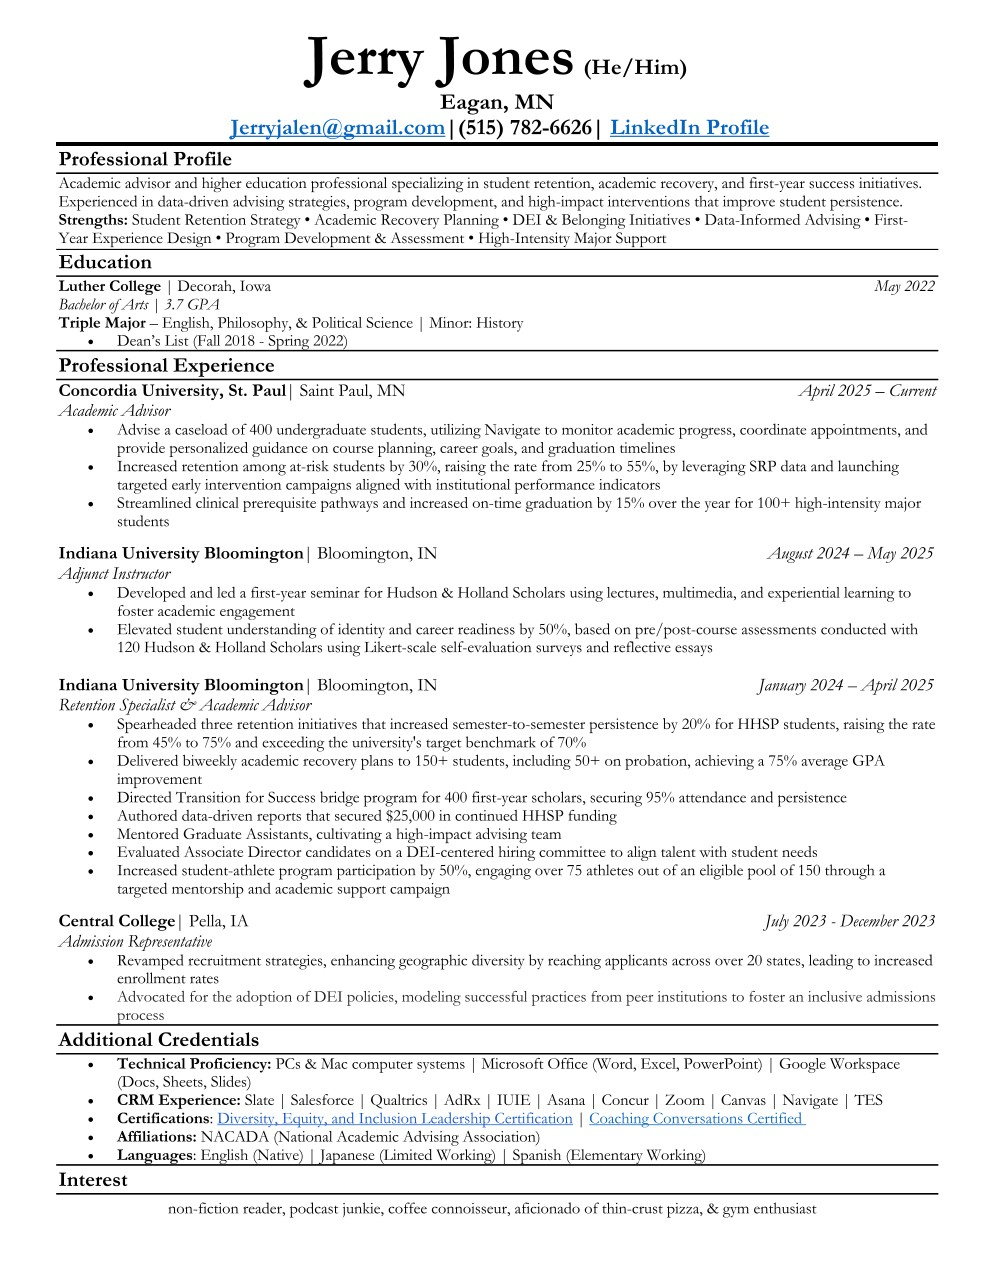
\includegraphics[width=\linewidth]{reference-resume-traditional-layout.jpeg}
    \caption{Reference: traditional one-column resume layout.}
\end{figure}

\begin{figure}[p]
    \centering
    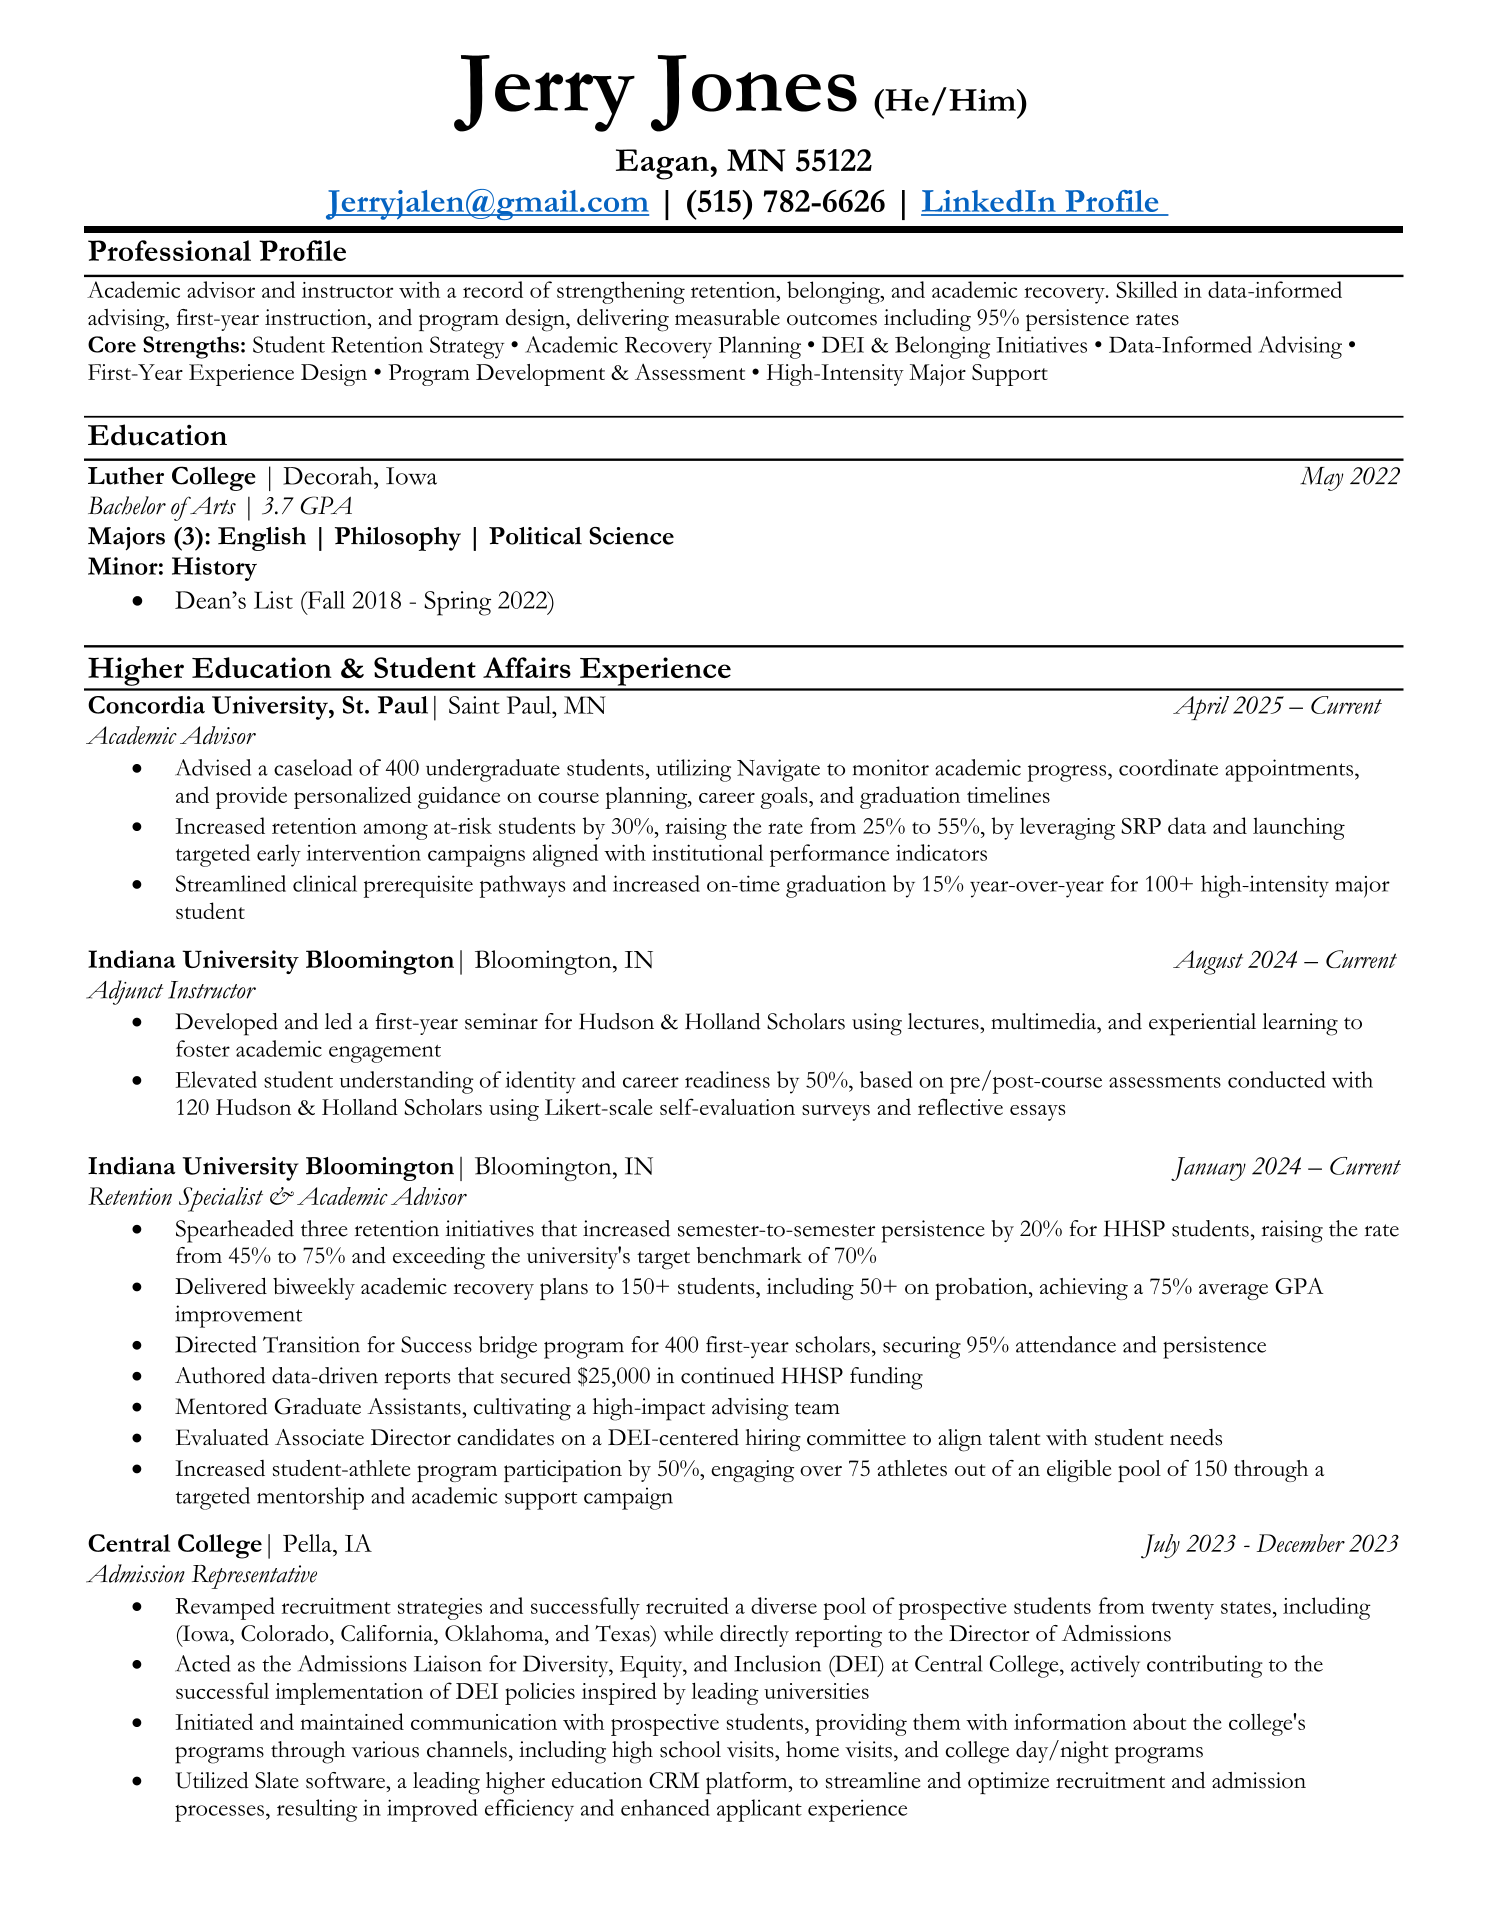
\includegraphics[width=\linewidth]{reference-resume-detailed-layout.png}
    \caption{Reference: resume with expanded experience section.}
\end{figure}

\begin{figure}[p]
    \centering
    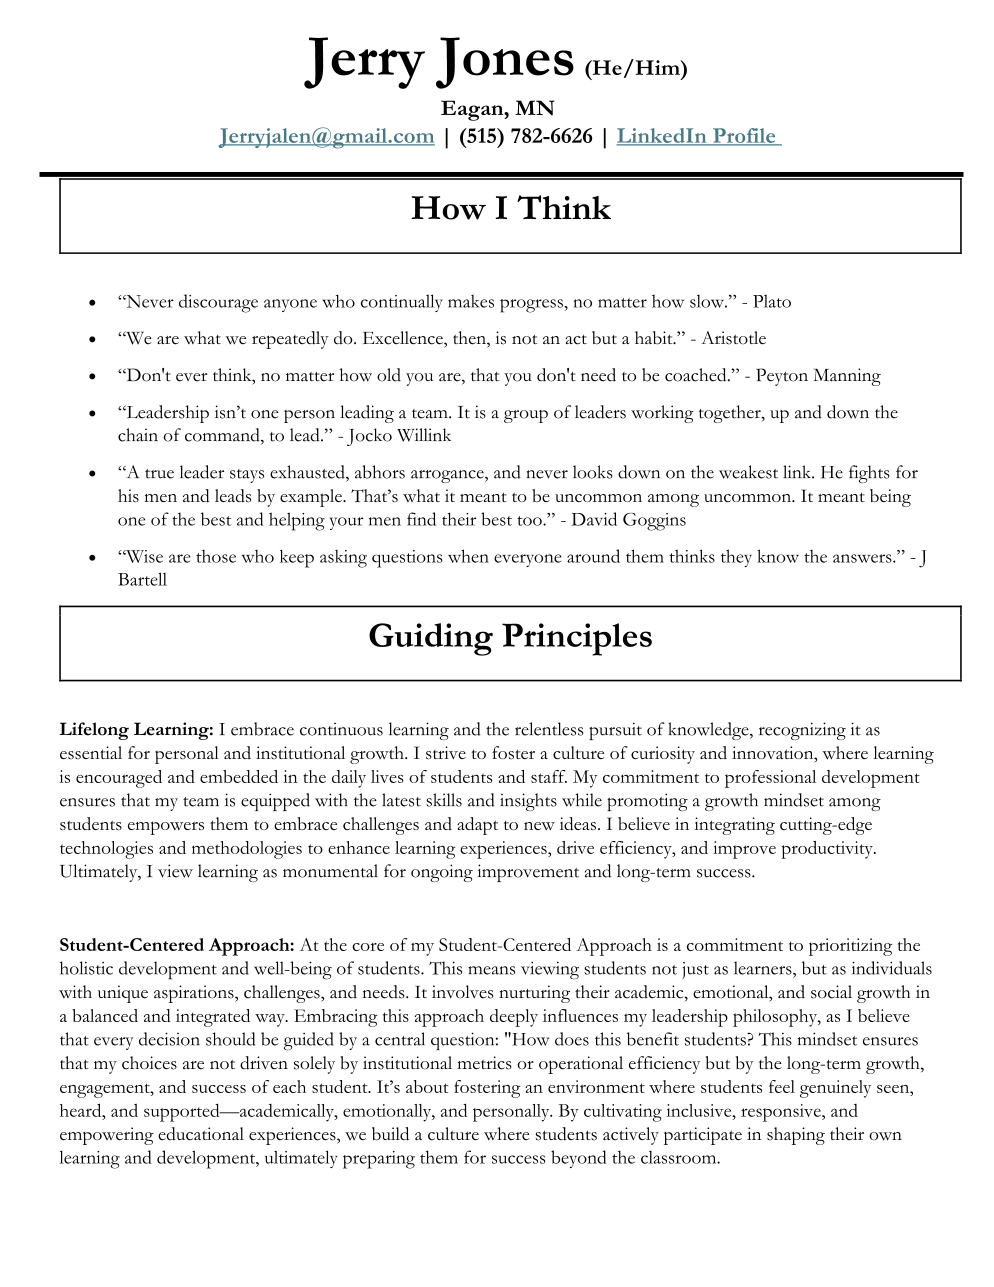
\includegraphics[width=0.95\linewidth]{reference-quotes-principles-layout.png}
    \caption{Reference: quotes + principles document.}
\end{figure}

\begin{figure}[p]
    \centering
    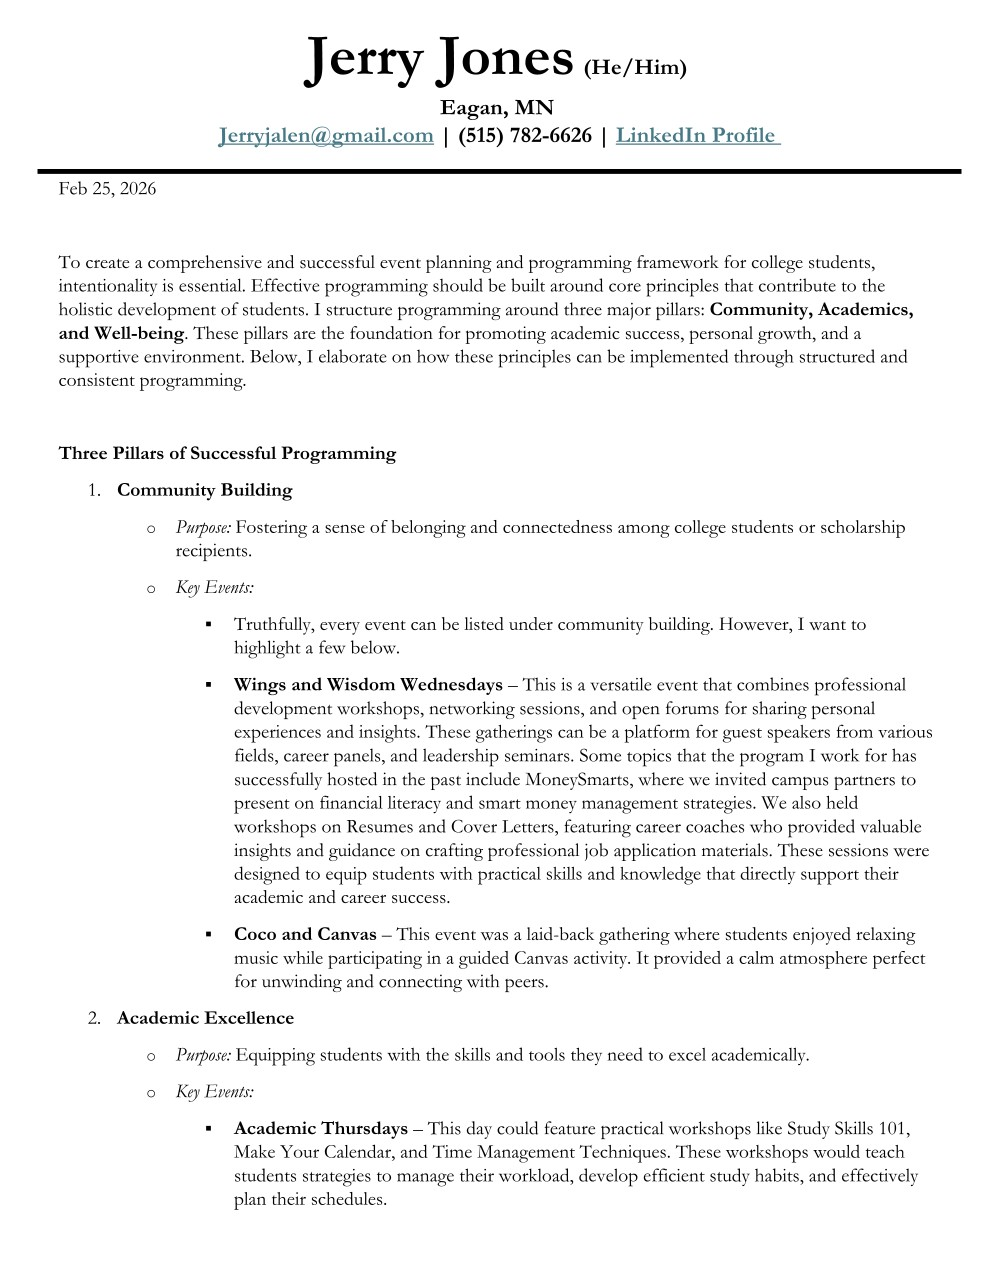
\includegraphics[width=\linewidth]{reference-three-pillars-programming-layout.jpeg}
    \caption{Reference: dated letter with numbered pillars.}
\end{figure}

\begin{figure}[p]
    \centering
    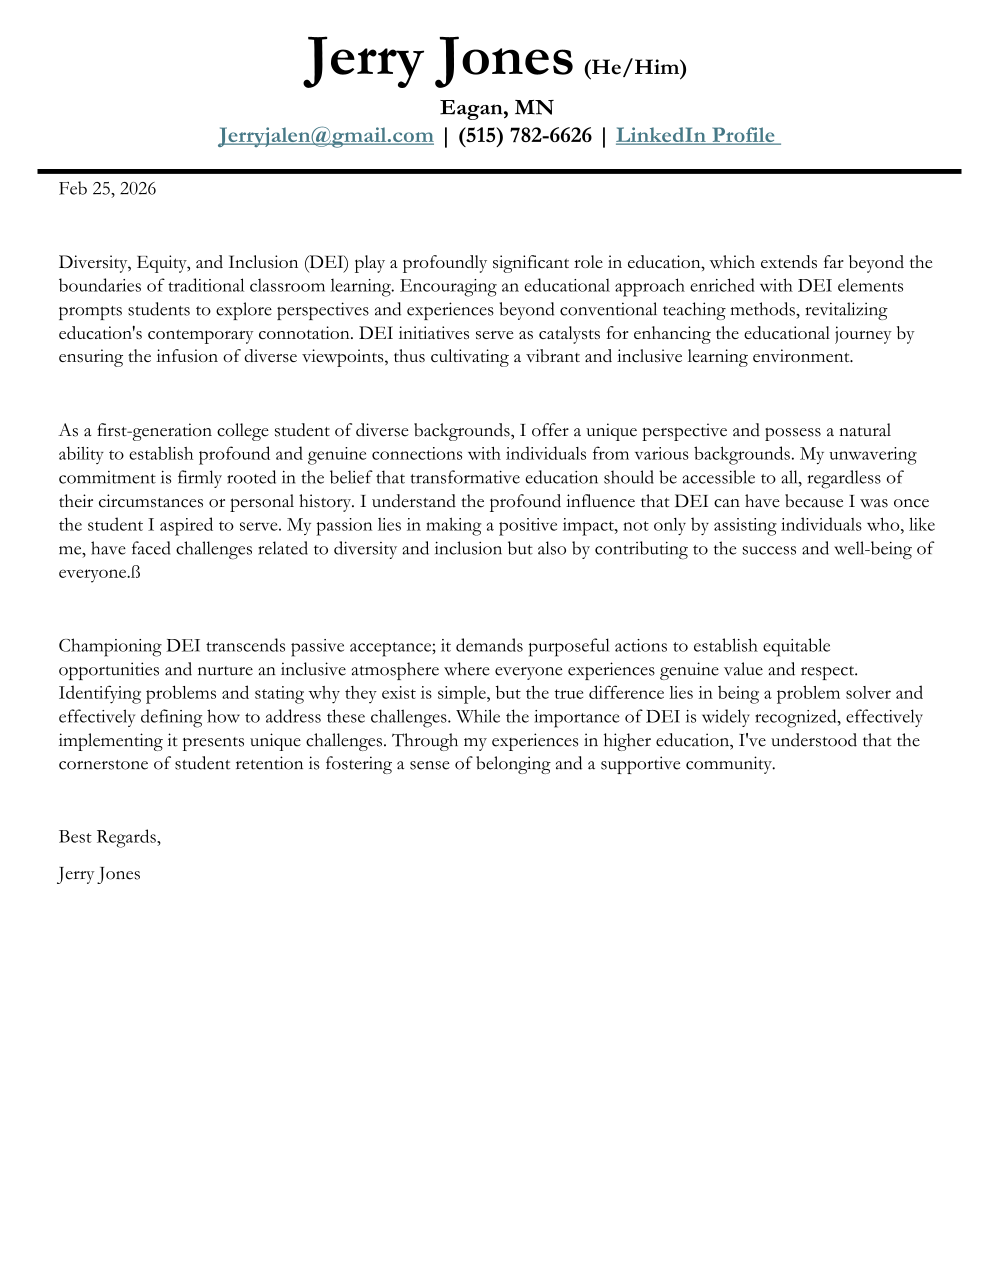
\includegraphics[width=\linewidth]{reference-dei-statement-layout.png}
    \caption{Reference: statement letter with rule below header.}
\end{figure}

\begin{figure}[p]
    \centering
    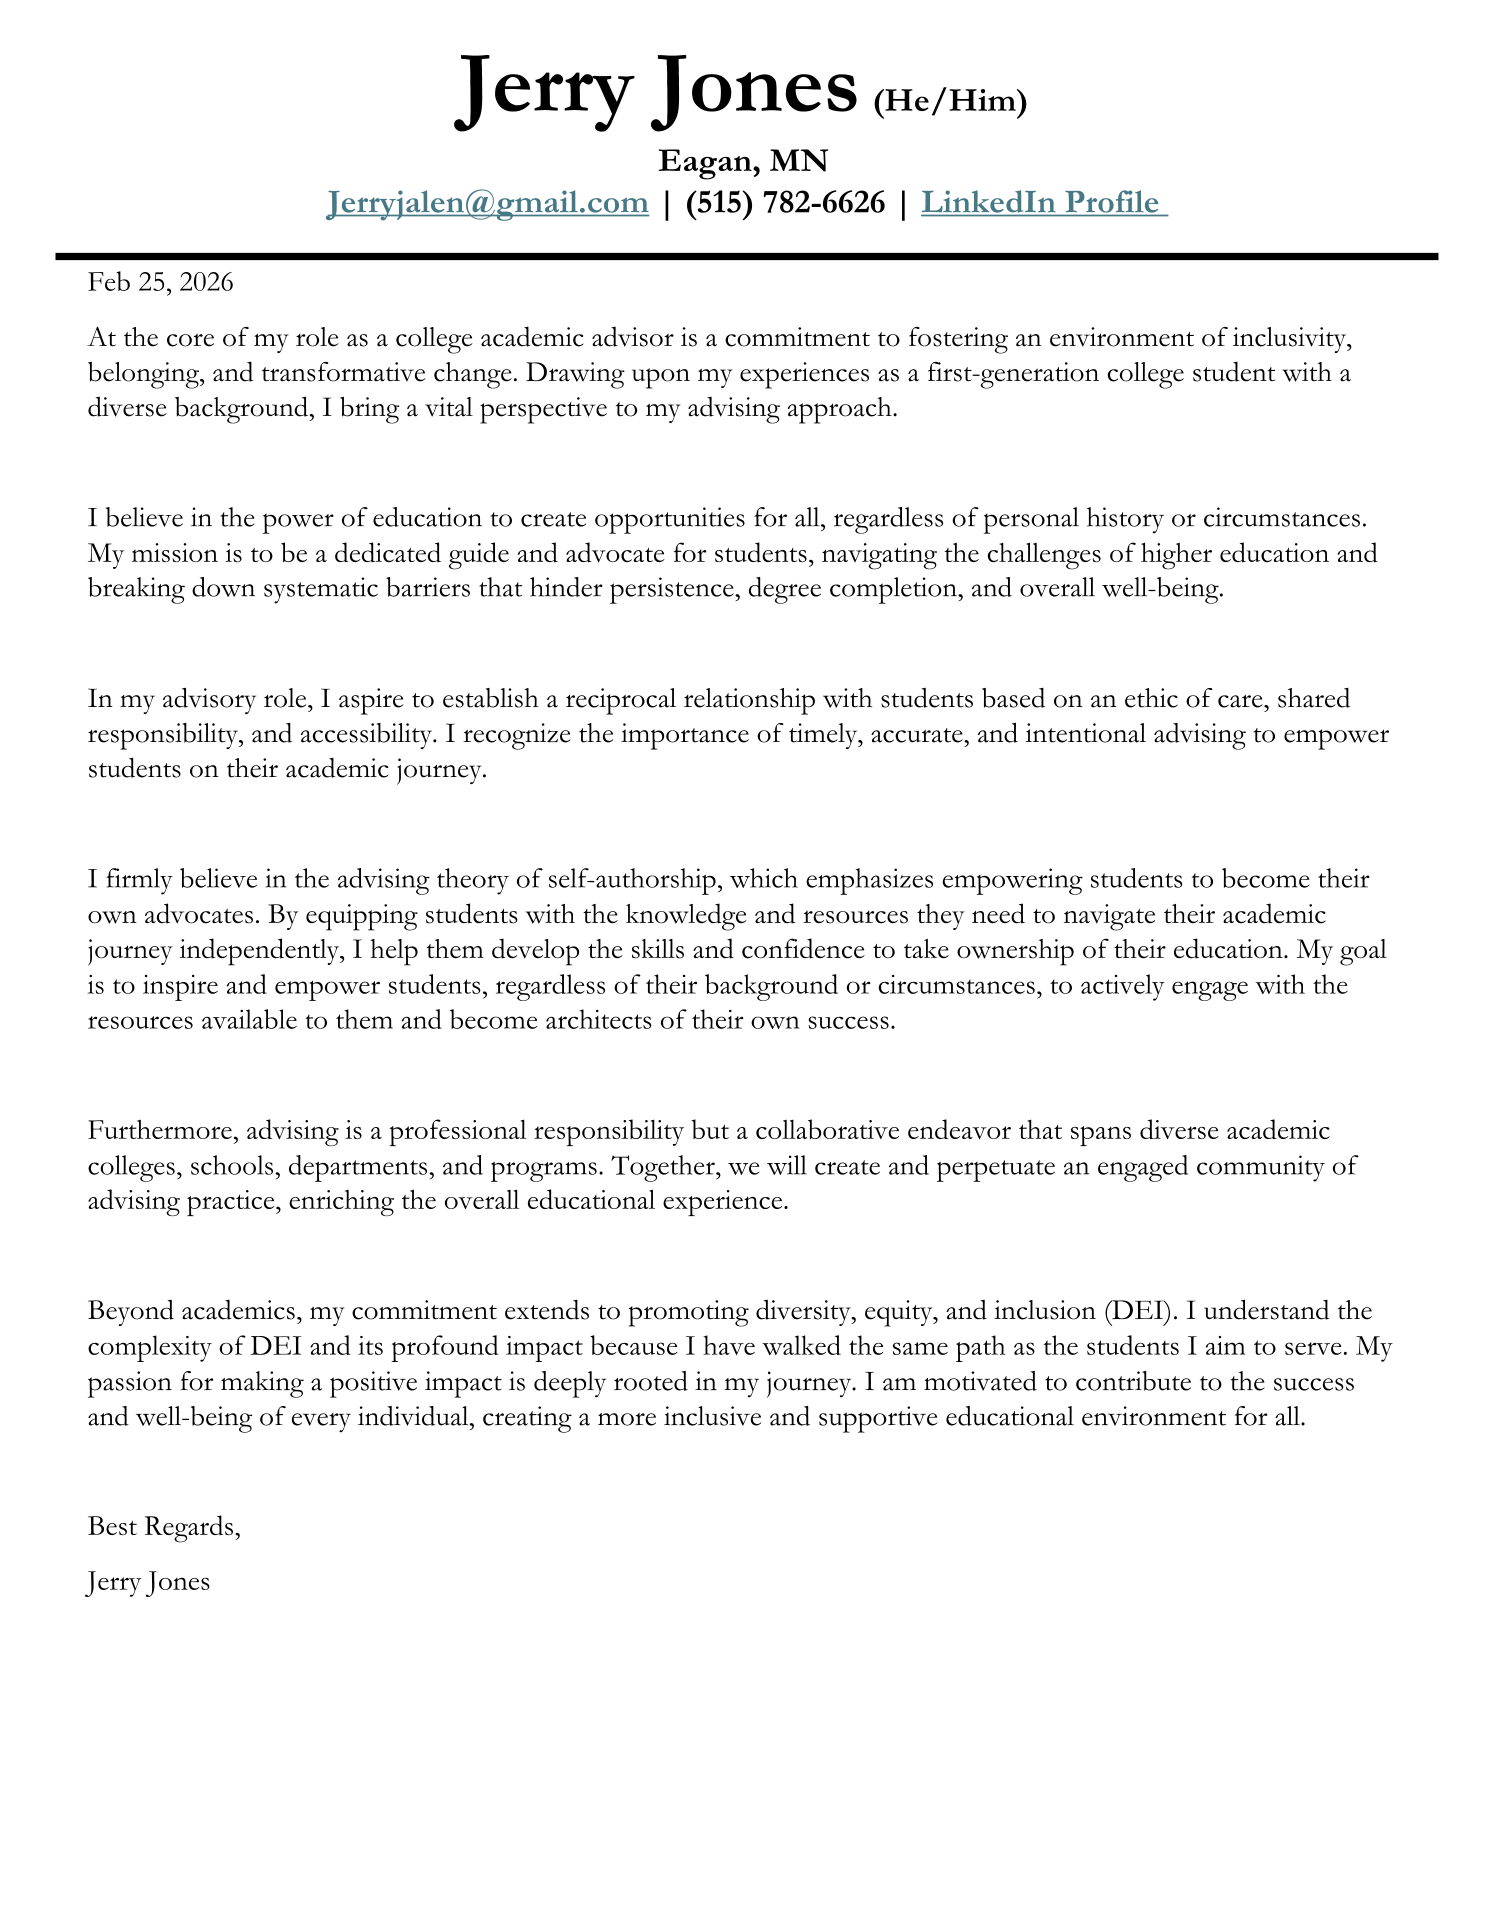
\includegraphics[width=\linewidth]{reference-philosophy-statement-layout.png}
    \caption{Reference: long-form philosophy statement.}
\end{figure}

\end{document}
